\hojaejercicio{Funciones Complejas y Ecuaciones Exponenciales}

% Ejercicio 4
\ejercicio{
Que le ocurre a la función $e^z$ en los siguientes conjuntos:
\begin{itemize}
    \item[a)] $ \{z\in\mathbb{C} \setminus \{0\}: |\arg(z)|<\frac{\pi}{2} - \delta, \delta>0\} = A$
    \item[b)] $ \{z\in\mathbb{C} \setminus \{0\}: \frac{\pi}{2} + \delta < \arg(z) < \frac{3\pi}{2} - \delta, \delta>0\} = B$
    \item[c)] $ \{z\in\mathbb{C} \setminus \{0\}: a \leq \Re(z) \leq b\}, a,b \in \mathbb{R} = C$
\end{itemize}
}{
    \begin{itemize}
        \item[a)] Tomemos la recta $y=\lambda_0 x$ con $\lambda_0=\tan(\frac{\pi}{2}-\delta)$, entonces:
        \[
        z \in A \implies
        x \to_{z \to \infty} +\infty \implies 
        |e^z| = e^x \to +\infty
        \]
        \item[b)] Tomemos la recta $y=\lambda_0 x$ con $\lambda_0=\tan(\frac{\pi}{2}+\delta)$, entonces:
        \[
        z \in B \implies
        x \to_{z \to \infty} -\infty \implies
        |e^z| = e^x \to 0
        \]
        \item[c)] Tenemos que $f(z) = e^z = e^{x+iy} = e^x(\cos(y) + i\sin(y))$, luego, como $y \to +\infty$ ó $y \to -\infty$, $e^z$ gira alrededor del origen con radio acotado entre $e^a$ y $e^b$.
        \begin{center}
            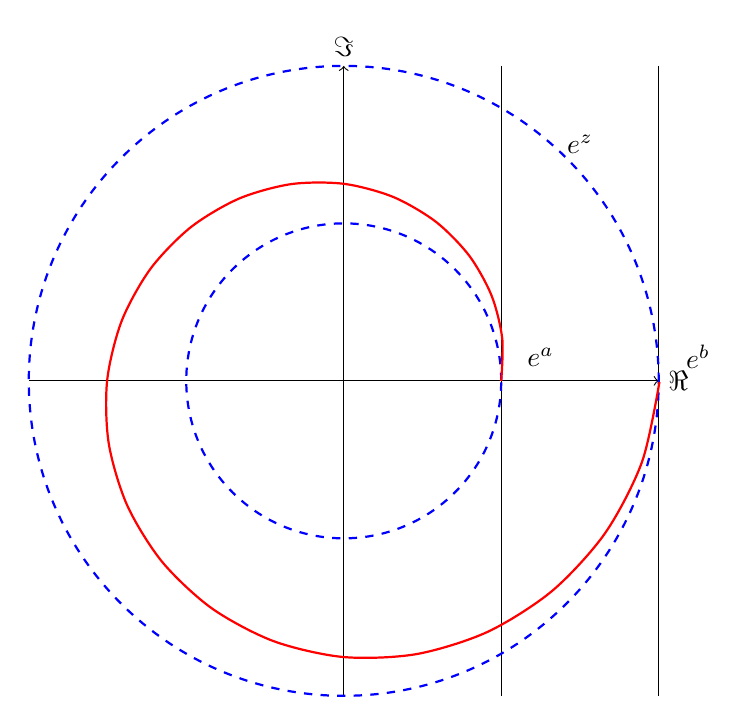
\begin{tikzpicture}
                % Ejes
                \draw[->] (-4,0) -- (4,0) node[right] {$\Re$};
                \draw[->] (0,-4) -- (0,4) node[above] {$\Im$};

                % Cilindro de a y b
                \draw[-] (2, - 4) -- (2, 4) node[above] {};
                \draw[-] (4, - 4) -- (4, 4) node[above] {};

                \draw[thick, dashed, blue] (0,0) circle (2);
                \draw[thick, dashed, blue] (0,0) circle (4);
                \node at (2.5,0.3) {$e^a$};
                \node at (4.5,0.3) {$e^b$};

                % Espiral
                \draw[thick, red, domain=0:6.28,smooth,variable=\t] plot ({(2 + 0.32*\t)*cos(\t r)}, {(2 + 0.32*\t)*sin(\t r)});
                \node at (3,3) {$e^z$};
            \end{tikzpicture}
        \end{center}
    \end{itemize}
}
\ejercicio{Determine los valores de $i^i$ y de $(-1)^{\sqrt{2}}$}{Para la base $z = i$:
\begin{itemize}
    \item \textbf{Módulo:} $|i| = 1$
    \item \textbf{Argumento principal:} $\theta = \frac{\pi}{2}$
    \item \textbf{Logaritmo:} $\ln(i) = \ln(1) + i\left(\frac{\pi}{2} + 2k\pi\right) = i\left(\frac{\pi}{2} + 2k\pi\right)$
\end{itemize}

Sustituyendo en la fórmula de la potencia:
\[ i^i = e^{i \cdot \ln(i)} = e^{i \cdot i\left(\frac{\pi}{2} + 2k\pi\right)} \]
\[ i^i = e^{-\left(\frac{\pi}{2} + 2k\pi\right)}, \quad k \in \mathbb{Z} \]



Para la base $z = -1$:
\begin{itemize}
    \item \textbf{Módulo:} $|-1| = 1$
    \item \textbf{Argumento principal:} $\theta = \pi$
    \item \textbf{Logaritmo:} $\ln(-1) = \ln(1) + i(\pi + 2k\pi) = i(2k+1)\pi$
\end{itemize}

Sustituyendo el exponente $w = \sqrt{2}$:
\[ (-1)^{\sqrt{2}} = e^{\sqrt{2} \cdot \ln(-1)} = e^{i\sqrt{2}(2k+1)\pi} \]

\textit{Nota: Dado que $\sqrt{2}$ es un número irracional, el conjunto de valores es infinito.}
}
\ejercicio{
    Resuelva $sen(z) = 2$
}{Sea $z = x + iy$. Expandimos el seno de una suma:
\[ \operatorname{sen} x \cosh y + i \cos x \sinh y = 2 \]

Igualamos las partes real e imaginaria:
\[ 
\begin{cases} 
(1) \quad \operatorname{sen} x \cosh y = 2 \\ 
(2) \quad \cos x \sinh y = 0 
\end{cases}
\]

De (2), dado que $\sinh y = 0 \implies y=0$ no satisface (1) (pues $\operatorname{sen} x \neq 2$), debe ser:
\[ \cos x = 0 \implies x = \frac{\pi}{2} + k\pi \]

Para que $\cosh y = \frac{2}{\operatorname{sen} x} > 0$, tomamos $x = \frac{\pi}{2} + 2k\pi$, donde $\operatorname{sen} x = 1$. Entonces:
\[ \cosh y = 2 \implies \frac{e^y + e^{-y}}{2} = 2 \]
\[ e^{2y} - 4e^y + 1 = 0 \implies e^y = 2 \pm \sqrt{3} \]
\[ y = \ln(2 \pm \sqrt{3}) \]

Entonces:
\[ z = \left( \frac{\pi}{2} + 2k\pi \right) + i \ln(2 \pm \sqrt{3}), \quad k \in \mathbb{Z} \]}
\ejercicio{}{1. Cálculo de $\operatorname{sen} i$:
Utilizando la relación $\operatorname{sen}(iz) = i \sinh z$:
\[ \operatorname{sen} i = i \sinh 1 = i \left( \frac{e - e^{-1}}{2} \right) \]

2. Cálculo de  $\cos i$:
Utilizando la relación $\cos(iz) = \cosh z$:
\[ \cos i = \cosh 1 = \frac{e + e^{-1}}{2} \]

3. Cálculo de $\operatorname{tg}(1+i)$:
Usamos la fórmula para la tangente de un número complejo $z = x + iy$:
\[ \operatorname{tg}(x + iy) = \frac{\operatorname{sen}(2x) + i \sinh(2y)}{\cos(2x) + \cosh(2y)} \]
Para $x=1$ e $y=1$:
\[ \operatorname{tg}(1+i) = \frac{\operatorname{sen} 2 + i \sinh 2}{\cos 2 + \cosh 2} \]}

\ejercicio{Encuentra las soluciones de las siguientes ecuaciones:}{
    Para resolver $e^z = w$, aplicamos $z = \ln|w| + i(\operatorname{Arg}(w) + 2k\pi)$, con $k \in \mathbb{Z}$.

\begin{enumerate}
    \item[a)] $e^z = 2 \implies z = \ln 2 + 2k\pi i$
    \item[b)] $e^z = -1 \implies z = i(\pi + 2k\pi) = (2k+1)\pi i$
    \item[c)] $e^z = i \implies z = i\left(\frac{\pi}{2} + 2k\pi\right) = \left(2k + \frac{1}{2}\right)\pi i$
    \item[d)] $e^z = -\frac{i}{2} \implies z = \ln\left(\frac{1}{2}\right) + i\left(-\frac{\pi}{2} + 2k\pi\right) = -\ln 2 + \left(2k - \frac{1}{2}\right)\pi i$
    \item[e)] $e^z = -1 \implies z = (2k+1)\pi i$
\end{enumerate}
}